\documentclass[11pt]{article}
\usepackage{preamble}

\newcommand{\IconCheck}{[CHECK]}
\newcommand{\IconMic}{[MIC]}
\newcommand{\IconClipboard}{[CLIPBOARD]}
\newcommand{\IconChart}{[CHART]}

\newcommand{\phasetag}[1]{%
  {\small\itshape Tag: #1\par}
}

\newcommand{\phaseitems}[1]{%
  \begin{itemize}[leftmargin=1.5em,itemsep=2pt,topsep=2pt]
  #1
  \end{itemize}%
}

\newcommand{\teacheranswerbox}[2]{%
  \begin{callout}{#1}{calloutgreen}
  #2
  \end{callout}
}

\newcommand{\entrybox}{\framebox[1.2em]{\rule{0pt}{0.95em}}}

\newcommand{\reciprocalblankgrid}{%
\begin{center}
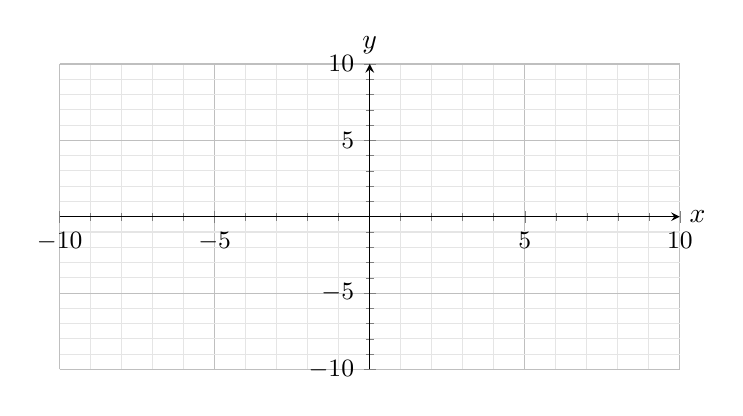
\begin{tikzpicture}
\begin{axis}[
  width=0.78\linewidth,
  height=2.15in,
  xmin=-10, xmax=10,
  ymin=-10, ymax=10,
  axis lines=middle,
  grid=both,
  minor tick num=4,
  xtick={-10,-5,0,5,10},
  ytick={-10,-5,0,5,10},
  tick label style={font=\small},
  label style={font=\small},
  major grid style={draw=black!25},
  minor grid style={draw=black!10},
  xlabel={$x$},
  ylabel={$y$},
  every axis x label/.style={at={(ticklabel* cs:1)},anchor=west},
  every axis y label/.style={at={(ticklabel* cs:1)},anchor=south}
]
\end{axis}
\end{tikzpicture}
\end{center}
}

\newcommand{\gamesblankgrid}{%
\begin{center}
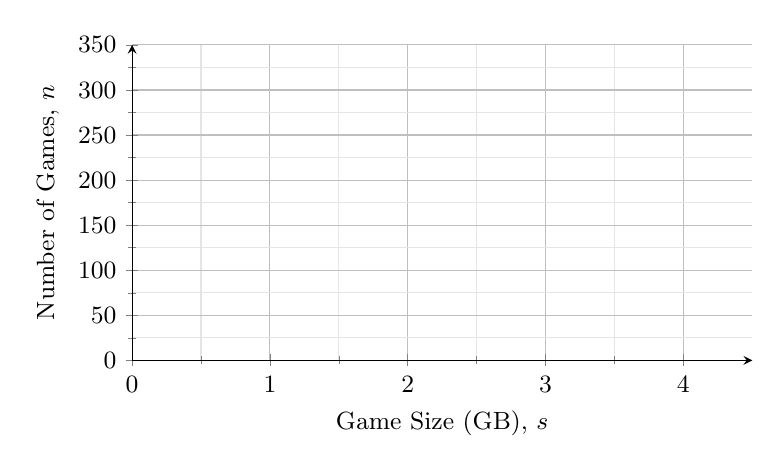
\begin{tikzpicture}
\begin{axis}[
  width=0.78\linewidth,
  height=2.2in,
  xmin=0, xmax=4.5,
  ymin=0, ymax=350,
  axis lines=left,
  grid=both,
  minor tick num=1,
  xtick={0,1,2,3,4},
  ytick={0,50,100,150,200,250,300,350},
  tick label style={font=\small},
  label style={font=\small},
  major grid style={draw=black!25},
  minor grid style={draw=black!10},
  xlabel={Game Size (GB), $s$},
  ylabel={Number of Games, $n$}
]
\end{axis}
\end{tikzpicture}
\end{center}
}

\newcommand{\qelevengraph}{%
\begin{center}
\begin{tikzpicture}
\begin{axis}[
  width=0.74\linewidth,
  height=2.65in,
  xmin=-6, xmax=6,
  ymin=-6, ymax=6,
  axis lines=middle,
  grid=both,
  minor tick num=1,
  xtick={-4,-2,0,2,4},
  ytick={-4,-2,0,2,4},
  tick label style={font=\small},
  label style={font=\small},
  major grid style={draw=black!25},
  minor grid style={draw=black!10},
  clip=false,
  xlabel={$x$},
  ylabel={$y$},
  every axis x label/.style={at={(ticklabel* cs:1)},anchor=west},
  every axis y label/.style={at={(ticklabel* cs:1)},anchor=south}
]
\addplot[warmred, thick, smooth] coordinates {(0.65,6) (1,5) (2,4) (5,1) (5.8,0.7)};
\addplot[warmred, thick, smooth] coordinates {(-5.8,-0.7) (-5,-1) (-2,-4) (-1,-5) (-0.65,-6)};
\addplot[only marks, mark=*, mark size=2.6pt, color=warmred] coordinates {
  (1,5) (2,4) (5,1) (-5,-1) (-2,-4) (-1,-5)
};
\node[text=warmred, anchor=west, font=\small\bfseries] at (axis cs:1.18,5.15) {\((1,5)\)};
\node[text=warmred, anchor=west, font=\small\bfseries] at (axis cs:2.22,4.15) {\((2,4)\)};
\node[text=warmred, anchor=west, font=\small\bfseries] at (axis cs:4.18,1.32) {\((5,1)\)};
\node[text=warmred, anchor=east, font=\small\bfseries] at (axis cs:-4.85,-1.15) {\((-5,-1)\)};
\node[text=warmred, anchor=east, font=\small\bfseries] at (axis cs:-1.78,-3.8) {\((-2,-4)\)};
\node[text=warmred, anchor=east, font=\small\bfseries] at (axis cs:-0.78,-5.1) {\((-1,-5)\)};
\node[text=warmred, font=\Large\bfseries] at (axis cs:4.35,-4.2) {X};
\end{axis}
\end{tikzpicture}
\end{center}
}

\begin{document}

\packetheading{Lesson 4-1 \textperiodcentered\ Period 3 \textperiodcentered\ Teacher Edition}{Reciprocal Function + Translations --- Assessment-Critical}

\sectionbanner{OBJECTIVES}
{\small
\renewcommand{\arraystretch}{1.25}
\noindent\begin{tabular}{|p{1.8in}|p{4.8in}|}
\hline
\textbf{Math Objective} & Graph the reciprocal function \(f(x) = 1/x\) and its translations \(g(x) = 1/(x-h) + k\). Identify vertical and horizontal asymptotes, state domain and range, and find intercepts where they exist. \\ \hline
\textbf{Language Objective} & Students will use the frame ``This graph is the parent \(f(x) = 1/x\) translated \_\_\_ units \_\_\_. The asymptotes are at \(x =\) \_\_\_ and \(y =\) \_\_\_.'' to describe any translated reciprocal function. \\ \hline
\textbf{Essential Understanding} & The reciprocal function has a vertical asymptote at \(x = 0\) and horizontal asymptote at \(y = 0\). Translations shift the asymptotes: \(g(x) = 1/(x-h) + k\) has asymptotes at \(x = h\) and \(y = k\). The point \((h, k)\) is the new ``center.'' \\ \hline
\end{tabular}
}

\sectionbanner{TOPIC GOALS / ESSENTIAL QUESTION / MATERIALS}
{\small
\renewcommand{\arraystretch}{1.25}
\noindent\begin{tabular}{|p{1.8in}|p{4.8in}|}
\hline
\textbf{Topic Goals} & Students will identify asymptotes and describe translations for 6 reciprocal-function items. This is Topic 4 assessment-prep material. \\ \hline
\textbf{Essential Question} & How do the values of \(h\) and \(k\) in \(g(x) = 1/(x-h) + k\) determine the graph's asymptotes, domain, range, and intercepts? \\ \hline
\textbf{Materials} & Pencils; student packet; graphing calculator (optional, for verification). \\ \hline
\end{tabular}
}

\begin{callout}{\IconPin\ PRE-FLIGHT --- P3 IS ASSESSMENT-CRITICAL}{calloutpink}
Topic 4 8-Q assessment Q\#3 (asymptotes) and Q\#5 (translation description) both come from Ex 4 + Ex 5 content. P3 is where students earn those 2 of 8 points.\\
Practice \#19 is THE rehearsal item: it has asymptotes + intercepts + implicit translation description.\\
No DOK-3 driver today (P2 owned the spine with \#26). P3 is pure DOK-2 mastery.\\
Pace: Try-It 4 (5) \(\rightarrow\) \#11 (5) \(\rightarrow\) \#18 (6) \(\rightarrow\) Try-It 5 (6) \(\rightarrow\) \#19 (8) \(\rightarrow\) \#21 (5). Total \(\sim\)35 min.\\
If pace slows: cut \#21 (modeling) first. Never cut \#19.
\end{callout}

\phasetag{bridge from P2}
\frameworkphaseheader{Do Now}{1}{5}{%
\phaseitems{
  \item Hand out at door.
  \item Circulate 3 min.
  \item Cold-call for two forms (\(y = k/x\) and \(xy = k\)).
}%
}{%
\phaseitems{
  \item Write \(k\) in both forms.
  \item Sketch prediction of \(y = 1/x\).
}%
}{%
\phaseitems{
  \item What ARE the two forms of inverse variation?
  \item Based on yesterday: predict what \(y = 1/x\) looks like.
}%
}{Solo teacher: circulate silently.}

\bankitem{Do Now --- Generalize: \(k\) in terms of \(x\) and \(y\)}{%
13. Generalize: For an inverse variation, write an equation that gives the value of \(k\) in terms of \(x\) and \(y\).
}{}

\teacheranswerbox{\IconCheck\ ANSWER KEY}{%
\textbf{Answer key (from TE):} \(k = xy\).
}

\begin{callout}{\IconSearch\ PREDICTION (spend 30 sec)}{calloutpeach}
Before we graph \(y = 1/x\) together, sketch what you THINK it looks like. (No wrong answers --- just predict.) We'll compare to the real thing in Launch.
\end{callout}

\sectionbanner{LAUNCH --- Reciprocal Function + Translations (teacher models Ex 4 + Ex 5)}

\phasetag{teacher models Ex 4 + Ex 5 back-to-back}
\frameworkphaseheader{Launch}{2}{12}{%
\phaseitems{
  \item FIRST 6 min: Example 4 --- graph \(f(x) = 1/x\). Emphasize asymptote behavior (approaching but never reaching). Show table of \(x \rightarrow 0\) and \(x \rightarrow \pm\infty\).
  \item NEXT 5 min: Example 5 --- graph \(g(x) = 1/(x-3) + 2\). Identify \((h, k) = (3, 2)\). Asymptotes shift accordingly.
  \item 30 sec: point at packet rule cards. ``Mark them. These are your assessment reference.''
  \item Do NOT solve Try-Its. Release at minute 17.
}%
}{%
\phaseitems{
  \item Watch Ex 4. Compare your Do Now prediction to the real graph.
  \item Watch Ex 5. Note: \(h\) shifts horizontal, \(k\) shifts vertical. \((h, k)\) is the new center.
  \item Copy BOTH rule cards into margins.
}%
}{%
\phaseitems{
  \item Why does \(y = 1/x\) never equal 0? (Because \(1/x = 0\) has no solution.)
  \item Why does \(x \neq 0\) in the domain? (Division by zero.)
  \item For \(g(x) = 1/(x-3) + 2\): what's \(h\)? What's \(k\)? Where do asymptotes cross?
  \item What happens as \(x \rightarrow 3\) from the right? From the left?
}%
}{Project both examples. Use a visible graphing tool (Desmos). Think aloud.}

\begin{callout}{\IconMic\ TEACHER SCRIPT}{calloutblue}
1. ``Yesterday we saw \(y = k/x\). Today we graph it and name its features.''\\
2. Example 4: ``As \(x\) gets huge (1000, 10000), \(y\) gets tiny (0.001, 0.0001) --- approaching ZERO but never reaching. That's a HORIZONTAL ASYMPTOTE at \(y = 0\).''\\
3. ``As \(x\) gets close to 0, \(y\) explodes --- POSITIVE infinity from the right, NEGATIVE infinity from the left. That's a VERTICAL ASYMPTOTE at \(x = 0\).''\\
4. Example 5: ``Now watch TRANSLATION. \(g(x) = 1/(x-3) + 2\). Subtract 3 inside \(\rightarrow\) shift RIGHT 3. Add 2 outside \(\rightarrow\) shift UP 2. New asymptotes: \(x = 3\), \(y = 2\).''\\
5. ``The POINT \((h, k)\) is the center of the translated graph. For \(g(x)\), center is \((3, 2)\).''\\
6. Release.
\end{callout}

\begin{callout}{\IconBook\ RECIPROCAL FUNCTION --- PARENT \(f(x) = 1/x\)}{calloutgreen}
\textbullet\ Vertical asymptote: \(x = 0\)\\
\textbullet\ Horizontal asymptote: \(y = 0\)\\
\textbullet\ Domain: \(\{x \mid x \neq 0\}\) \hspace{1.8em} \textbullet\ Range: \(\{y \mid y \neq 0\}\)\\
\textbullet\ Graph: hyperbola in Quadrants I and III (two branches, no intersection)
\end{callout}

\begin{callout}{\IconBook\ TRANSLATED RECIPROCAL --- \(g(x) = 1/(x-h) + k\)}{calloutyellow}
\textbullet\ Vertical asymptote shifts to: \(x = h\)\\
\textbullet\ Horizontal asymptote shifts to: \(y = k\)\\
\textbullet\ Domain: \(\{x \mid x \neq h\}\) \hspace{1.8em} \textbullet\ Range: \(\{y \mid y \neq k\}\)\\
\textbullet\ The point \((h, k)\) is the ``new center'' --- where the asymptotes cross.\\
\textbullet\ Example: \(g(x) = 1/(x-3) + 2\) \(\rightarrow\) asymptotes \(x = 3\) and \(y = 2\).

\medskip
To find INTERCEPTS:\\
\hspace*{1.5em}\textbullet\ y-intercept: set \(x = 0\). \(y = 1/(0-h) + k = -1/h + k.\)\\
\hspace*{1.5em}\textbullet\ x-intercept: set \(y = 0\). Solve \(0 = 1/(x-h) + k \rightarrow x = h - 1/k.\)
\end{callout}

\sectionbanner{EXPLORE --- Think-Pair-Share (35 min)}

\phasetag{TPS --- pure DOK-2 mastery --- assessment rehearsal}
\frameworkphaseheader{Explore}{2}{35}{%
\phaseitems{
  \item 6 laps across 35 min.
  \item Laps 1-3: Try-It 4 + \#11 + \#18. Parent-form scaled/reflected. (5-6 min each.)
  \item Laps 4-5: Try-It 5 + \#19 --- translated forms. \#19 is the assessment rehearsal --- press on BOTH asymptotes AND intercepts.
  \item Lap 6: \#21 --- modeling. If time.
  \item Do not give answers. Use sentence frame to press justification.
}%
}{%
\phaseitems{
  \item 6 items in order. Parent forms first (Try-It 4, \#11, \#18), then translations (Try-It 5, \#19, \#21).
  \item For \#19: BEFORE graphing, state \((h, k)\), asymptotes, and domain/range.
  \item Justify with sentence frame.
}%
}{%
\phaseitems{
  \item What's the center of the translation? \((h, k)\)
  \item Which asymptote is which? (\(x = h\) vertical; \(y = k\) horizontal.)
  \item For \#11: what \(y\)-value does \(y = 5/x\) actually give at \(x = 2\)? (2.5 --- the labeled 4 is wrong.)
  \item For \#18: how does the negative flip the graph? (Quadrants II and IV instead of I and III.)
  \item For \#19: what are the asymptotes? What are the intercepts?
}%
}{Solo teacher: 6 laps. Press BOTH asymptotes AND intercepts on \#19. This IS the assessment rehearsal.}

\textbf{Bank-item labels (in order):}
\begin{enumerate}[leftmargin=1.6em,itemsep=2pt,topsep=2pt]
  \item Try It 4 --- Graph \(g(x) = 10/x\) (scaled parent)
  \item Practice \#11 --- Error Analysis: \(y = 5/x\)
  \item Practice \#18 --- Graph \(y = -2/x\) (reflected parent)
  \item Try It 5 --- Graph \(g(x) = 1/(x+2) - 4\) (translated)
  \item Practice \#19 \IconStar\ ASSESSMENT CRITICAL --- \(g(x) = 1/(x-2) + 6\) + intercepts
  \item Practice \#21 --- Video game storage (modeled)
\end{enumerate}

\bankitem{Try It 4 --- Graph \(g(x) = 10/x\) (scaled parent)}{%
Try It 4. Graph the function \(g(x) = 10/x\). What are the domain, range, and asymptotes of the function?
\reciprocalblankgrid
}{}

\teacheranswerbox{\IconCheck\ ANSWER / ANTICIPATED TALK}{%
\textbf{Answer key (from TE):} graph passes through \((1,10)\), \((10,1)\), \((-10,-1)\), \((-1,-10)\); domain: all real numbers, \(x \neq 0\); range: all real numbers, \(y \neq 0\); horizontal asymptote \(y = 0\); vertical asymptote \(x = 0\). Graph of \(g(x) = 10/x\) is a vertical stretch of \(f(x) = 1/x\).
}

\bankitem{Practice \#11 --- Error Analysis: \(y = 5/x\)}{%
11. Error Analysis: Describe and correct the error a student made in graphing the function \(y = 5/x\). The student's graph shows labeled points \((1, 5)\), \((2, 4)\), \((5, 1)\) in Quadrant I and \((-5, -1)\), \((-2, -4)\), \((-1, -5)\) in Quadrant III, with a large red X indicating the graph is incorrect.
\qelevengraph
}{}

\teacheranswerbox{\IconCheck\ ANSWER / ANTICIPATED TALK}{%
\textbf{Answer key (from TE):} The points \((2, 4)\) and \((-2, -4)\) are not correct. The labels of these points should be \((2, 2.5)\) and \((-2, -2.5)\). Reason: \(y = 5/2 = 2.5\), not 4.
}

\bankitem{Practice \#18 --- Graph \(y = -2/x\) (reflected parent)}{%
18. Graph the function \(y = -2/x\). What are the domain, range, and asymptotes of the function?
\reciprocalblankgrid
}{}

\teacheranswerbox{\IconCheck\ ANSWER / ANTICIPATED TALK}{%
\textbf{Answer key (from TE):} vertical asymptote: \(x = 0\); horizontal asymptote: \(y = 0\); domain: the set of real numbers except 0 (\(x \neq 0\)); range: the set of real numbers except 0 (\(y \neq 0\)). The graph is the reciprocal function reflected over the \(x\)-axis (Quadrants II and IV) and vertically stretched by a factor of 2.
}

\bankitem{Try It 5 --- Graph \(g(x) = 1/(x+2) - 4\) (translated)}{%
Try It 5. Graph \(g(x) = 1/(x + 2) - 4\). What are the equations of the asymptotes? What are the domain and range?
\reciprocalblankgrid
}{}

\teacheranswerbox{\IconCheck\ ANSWER / ANTICIPATED TALK}{%
\textbf{Answer key (from TE):} vertical asymptote \(x = -2\); horizontal asymptote \(y = -4\); domain: set of real numbers with \(x \neq -2\); range: set of real numbers with \(y \neq -4\). Graph translated 2 units left and 4 units down from parent.
}

\bankitem{Practice \#19 \IconStar\ ASSESSMENT CRITICAL --- \(g(x) = 1/(x-2) + 6\) + intercepts}{%
19. Graph \(g(x) = 1/(x - 2) + 6\). What are the equations of the asymptotes? What are the domain and range? What are the intercepts?
\reciprocalblankgrid
}{}

\teacheranswerbox{\IconCheck\ ANSWER / ANTICIPATED TALK}{%
\textbf{Answer key (from TE):} vertical asymptote \(x = 2\); horizontal asymptote \(y = 6\); domain: set of real numbers with \(x \neq 2\); range: set of real numbers with \(y \neq 6\); \(y\)-intercept: \(5.5\) (or \(11/2\)); \(x\)-intercept: \(11/6\). Graph shows translated reciprocal function with asymptotes intersecting at \((2, 6)\).
}

\bankitem{Practice \#21 --- Video game storage (modeled)}{%
21. Use Structure: The number of downloaded games that can be stored on a video game system varies inversely with the average size of a video game. A certain video game system can store 160 games when the average size of a game is 2.0 gigabytes (GB). (a) Write an inverse equation that relates the number of games \(n\) that will fit on the video game system as a function of the average game size \(s\) in GB. (b) Use the inverse relationship to complete the table of values. Game Size (GB), \(s\): 1.0, 2.5, 3.0, 4.0; Number of Games, \(n\): \_, \_, \_, \_. (c) Sketch a graph of this inverse relationship on a coordinate plane.
\begin{center}
\renewcommand{\arraystretch}{1.35}
\begin{tabular}{|l|c|c|c|c|}
\hline
\textbf{Game Size (GB), \(s\)} & 1.0 & 2.5 & 3.0 & 4.0 \\ \hline
\textbf{Number of Games, \(n\)} & \entrybox & \entrybox & \entrybox & \entrybox \\ \hline
\end{tabular}
\end{center}
\gamesblankgrid
}{}

\teacheranswerbox{\IconCheck\ ANSWER / ANTICIPATED TALK}{%
\textbf{Answer key (from TE):} (a) \(n = 320/s\) (since \(k = 160 \cdot 2.0 = 320\)). (b) Table values: \(s = 1.0 \rightarrow n = 320\); \(s = 2.5 \rightarrow n = 128\); \(s = 3.0 \rightarrow n = 106.7\); \(s = 4.0 \rightarrow n = 80\). (c) Hyperbola through labeled points \((1, 320)\), \((2, 160)\) in Quadrant I and \((-1, -320)\), \((-2, -160)\) in Quadrant III (though physical context only supports Quadrant I).
}

\sectionbanner{SHARE / SUMMARY (5 min)}

\phasetag{Concept Summary + LEHS 8-Q preview}
\frameworkphaseheader{Share / Summary}{2}{5}{%
\phaseitems{
  \item Cold-call 1 pair to present \#19 (asymptotes + intercepts).
  \item Project Concept Summary (from student packet).
  \item ``Topic 4 8-Q assessment: expect 2 of 8 questions on THIS content --- asymptotes and translation descriptions. You just rehearsed both.''
}%
}{%
\phaseitems{
  \item Presenting pair uses sentence frame for \#19.
  \item Rest of class signals and annotates their Concept Summary.
}%
}{%
\phaseitems{
  \item What are the TWO big ideas from Lesson 4-1?
  \item If you see \(g(x) = a/(x-h) + k\) on the assessment, what's the FIRST thing you identify?
}%
}{Frame today as assessment rehearsal. Students leave confident.}

\begin{sentenceframebox}
\textbf{Sentence frames}

Pair share (\#19): ``This graph is the parent \(f(x) = 1/x\) translated \_\_\_ units \_\_\_ and \_\_\_ units \_\_\_. The asymptotes are \(x =\) \_\_\_ and \(y =\) \_\_\_. The intercepts are \_\_\_.''

Whole class: one pair reads \#19. Class signals thumbs up/sideways.
\end{sentenceframebox}

\begin{callout}{\IconChart\ CONCEPT SUMMARY (your reference for Topic 4 assessment)}{calloutell}
INVERSE VARIATION (\(y = k/x\)):\\
\hspace*{1.5em}--- WORDS: As one variable increases, the other decreases; their product \(k\) is constant.\\
\hspace*{1.5em}--- ALGEBRA: \(y = k/x\) where \(k \neq 0\)\\
\hspace*{1.5em}--- GRAPH: parent hyperbola, asymptotes \(x = 0\) and \(y = 0\)

\medskip
RECIPROCAL FUNCTION TRANSLATIONS (\(y = a/(x-h) + k\)):\\
\hspace*{1.5em}--- WORDS: The reciprocal function can shift left/right (\(h\)) and up/down (\(k\)).\\
\hspace*{1.5em}--- ALGEBRA: \(y = a/(x-h) + k\)\\
\hspace*{1.5em}--- GRAPH: asymptotes shift to \(x = h\) and \(y = k\); new ``center'' at \((h, k)\).
\end{callout}

\sectionbanner{EXIT TICKET}

\phasetag{pre-assessment confidence check}
\frameworkphaseheader{Exit Ticket}{1-2}{3}{%
\phaseitems{
  \item Collect at door.
  \item Tonight: scan confidence scores. If averages <3 on asymptotes or translations, insert a 5-min Do Now recap when the 8-Q lands.
}%
}{%
\phaseitems{
  \item Rate own confidence 1-5 on two skills.
  \item Name one thing to review.
}%
}{%
\phaseitems{
  \item Did any student score <3 on either skill?
  \item What specific content did students name wanting to review?
}%
}{Collect. No grade. Use as data for future assessment prep.}

\begin{callout}{\IconClipboard\ EXIT TICKET --- Student Form}{calloutyellow}
I can identify asymptotes of \(y = 1/(x-h) + k\).     Confidence: 1 / 2 / 3 / 4 / 5\\
I can describe a translation from \(f(x) = 1/x\) to \(g(x)\).     Confidence: 1 / 2 / 3 / 4 / 5\\
One thing I want to review before Topic 4 assessment: \_\_\_.
\end{callout}

\sectionbanner{OPTIONAL REINFORCEMENT (not collected)}
\textit{Extra stretch for fast finishers. Try without a calculator first.}

\bankitem{Optional \#1  (Savvas SAT/ACT style)}{%
25. SAT/ACT. In a given set of experiments, \(t\) and \(w\) always vary inversely. When \(t = 0.4\) seconds, \(w = 172.8\) grams. How much time has passed when \(w = 14.4\) grams?
}{%
  \answerchoice{A}{2.4 s}
  \answerchoice{B}{4.8 s}
  \answerchoice{C}{27.648 s}
  \answerchoice{D}{995.328 s}
}

\teacheranswerbox{\IconCheck\ ANSWER / ANTICIPATED TALK}{%
\textbf{Correct answer:} B) 4.8 s (confirmed by TE answer key with filled circle on B).
}

\clearpage

\begin{callout}{\IconClock\ PERIOD A / PERIOD F --- 65-MIN CLASS NOTES}{calloutpink}
Both sections should have 65 min. Use extra 10 min on Explore \#19 (assessment-critical).\\
If finished early: Practice \#25 (SAT/ACT MC) as fast-finisher stretch.\\
Alternative: project Practice \#11 as a second Error Analysis prompt --- more asymptote practice.
\end{callout}

\begin{callout}{\IconPuzzle\ MODIFICATIONS / SUPPORT FOR IEP STUDENTS}{calloutiep}
\textbullet\ Provide both Rule cards as half-sheet cut-outs on their desks.\\
\textbullet\ For \#19, provide a pre-axed grid (labeled \(x\) and \(y\) from -4 to 8) so they don't spend time drawing axes.\\
\textbullet\ Accept verbal asymptote identification in lieu of written.
\end{callout}

\begin{callout}{\IconGlobe\ SUPPORTS FOR ELL STUDENTS}{calloutell}
\textbullet\ Sentence frames on student page (don't skip).\\
\textbullet\ Word cards: ``asymptote'' = line the graph approaches but never touches.\\
\textbullet\ ``reciprocal'' = the fraction flipped; \(1/x\) is the reciprocal of \(x\).\\
\textbullet\ ``translation'' = shift of the whole graph (no rotation or resize).\\
\textbullet\ Pair ELL students with English-dominant partners for TPS.
\end{callout}

\end{document}
